\chapter{Testing for Verification}\label{ch:verification}

This chapter addresses verification, that is, whether the code solves the stated
equations correctly. The comparison of the surrogate with direct RVE solutions is
presented in \cref{ch:assessment}; experimental validation was not part of the
project.

All tests use the production modules; no routine exists in a separate test copy.
The tests were run during development (Phase~1 locally, Phase~2 on the cluster)
and, for the final code state, the complete suite was executed with the frozen
checkpoints and datasets (Python~3.13.18, NGSolve~6.2.2608, PyTorch~2.15.0). All
tests passed; the values below are from this execution. The complete suite runs with one command
(\code{./run\_tests.sh}, \cref{ch:manual}). \Cref{tab:vmatrix} gives the overview. Guideline items that do not
apply are stated explicitly: the model is quasi-static and rate-independent, so
there is no time integration and the time-integration stability and
convergence-order tests are not applicable.

{\small
\begin{xltabular}{\textwidth}{@{}llXl@{}}
\caption[Verification matrix (26 tests)]{Verification matrix (26 tests). Type: M = mandatory test of the guideline,
S = standard benchmark, C = custom (project-specific). All tests passed.}\label{tab:vmatrix}\\
\toprule
ID & Type & Aim & Key result\\
\midrule
\endfirsthead
\caption[]{\emph{(continued)}}\\
\toprule
ID & Type & Aim & Key result\\
\midrule
\endhead
\bottomrule
\endfoot
V0a & M & partition of unity of the shape functions ($P_1$, $P_2$) & $|\sum N_i-1|\le2.2\times10^{-16}$\\
V0b & M & exact linear field and gradient ($B$-matrix check) & gradient error $\le4.0\times10^{-14}$\\
V0c & M & volume/area by quadrature of the Jacobian, affine map & error $2.2\times10^{-14}$\\
V0d & M & six zero eigenvalues of the element stiffness (tet, hex; $P_1$, $P_2$) & 6/6 zero modes, span error $\le2\times10^{-9}$\\
V0e & M & hourglass modes under one-point integration & 18 zero modes (6 rigid + 12)\\
V1 & C & constitutive API, shapes, dtypes & pass\\
V2 & C & $\widehat\Psi(\Iten)=0$, $\Pstress(\Iten)=\bm 0$ & exactly $0$\\
V2b & S & pICNN vs.\ analytical neo-Hookean response & $5.37/3.27/3.87\,\%$\\
V3 & M & AD tangent vs.\ central differences & min.\ error $2.3\times10^{-10}$\\
V4 & M & Newton convergence, nonlinear FE solve & empirical order $1.90$\\
V5 & M & affine patch test, unstructured mesh & $\|\bm R_\mathrm{free}\|=2.7\times10^{-16}$\\
V6 & S & matched analytical vs.\ neural FE solution & reaction error $13.4\,\%<15\,\%$\\
V7 & M & single element, full deformation control: stress and tangent (SVK, neo-Hooke) & stress $5.5\times10^{-15}$, tangent $1.7\times10^{-11}$\\
V8 & M & single element, stress control (uniaxial traction), SVK then neo-Hooke & stretches exact to $2\times10^{-15}$\\
P2-V1 & C & triple periodicity of the fluctuation space & jump $2.2\times10^{-16}$\\
P2-V2 & C & exact rigid kinematics (rank 6, finite rotation) & constraint residual $7.2\times10^{-18}$\\
P2-V3 & M & mixed patch at $\kappa/\mu=10^4$ & $p$ error $2.9\times10^{-13}$\\
P2-V4 & C & coupled periodic RVE equilibrium & residual $1.9\times10^{-14}$\\
P2-V5 & S & Hill--Mandel macro-homogeneity & $1.2\times10^{-15}$\\
P2-V6 & M & condensed tangent: symmetry, Taylor order & order $2.000$, sym.\ $3.0\times10^{-16}$\\
P2-V7 & C & free rotation: moment equilibrium, $\Rten\in SO(3)$ & 3 iterations, $\|\Rten^{\mathsf T}\Rten-\Iten\|=2.5\times10^{-16}$\\
P2-V8 & C & translation-gauge invariance & stress change $1.2\times10^{-15}$\\
P2-V9 & M & free-rotation tangent vs.\ re-solved central differences & error $5.2\times10^{-12}$\\
P2-V10 & C & deterministic dataset, leak-free splits & 0 leaks, regeneration error $0$\\
S-V1 & M & surrogate: energy gradient, tangent, objectivity & $\le4.9\times10^{-8}$\\
M-V0 & M & macroscopic tangent vs.\ directional differences & $6.5\times10^{-10}$\\
\end{xltabular}
}

\Cref{fig:voverview} plots the key error measure of every test on one scale.
Most tests reach round-off ($10^{-18}$--$10^{-13}$), because they check an
identity that holds exactly in exact arithmetic. Larger values appear only where
the test measures an approximation or a tolerance by design: the trained Phase~1
network against the analytical law (V2b, V6); finite differences against an exact
derivative (V3, P2-V9, S-V1, M-V0), whose error is set by the difference step; the
Newton stopping tolerance (V4); and the eigenvalue threshold that defines the
numerical null space (V0d). The boundary-value problem of each element-level test is drawn
next to its description; the RVE tests use the model of \cref{fig:rvesetup}.

\begin{figure}[H]
\centering
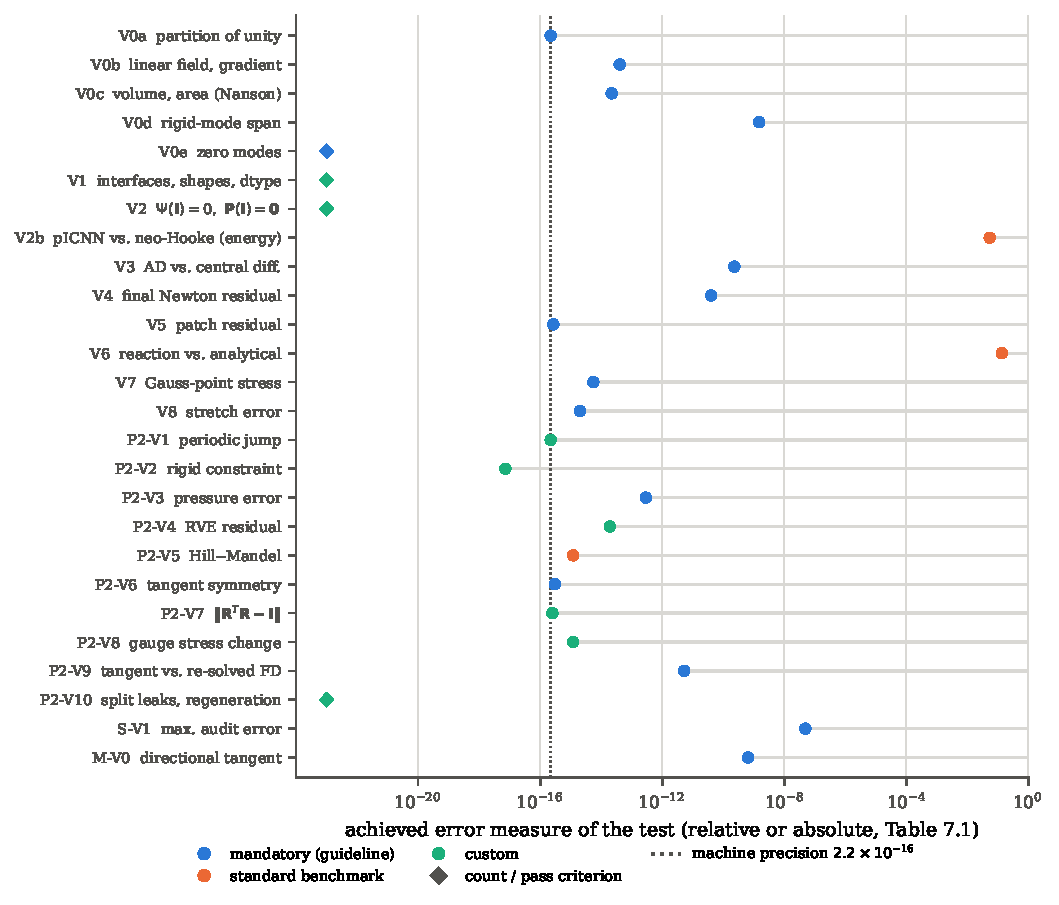
\includegraphics[width=\textwidth]{fig_v_overview.pdf}
\caption[Key error measure of all 26 verification tests]{Key error measure of all 26 verification tests (\cref{tab:vmatrix}).
Diamonds: tests with a count or a pass criterion instead of an error measure.
Dotted: machine precision $2.2\times10^{-16}$.}
\label{fig:voverview}
\end{figure}

% ======================================================================
\section{Finite-element basics}\label{sec:v0}

The NGSolve element library is heavily tested by its developers. The guideline
nevertheless requires these checks, because they also exercise \emph{this}
project's assembly path. All five are implemented in
\code{tests\slash{}verify\_fe\_basics.py} and use the production routine
\code{assemble\_system}.

\testcase{V0a/V0b}{Partition of unity and exact representation of linear fields}
\taim Verify $\sum_iN_i=1$ and $\sum_i\nabla N_i=\bm 0$, and that a linear field
and its gradient are reproduced exactly, for $P_1$ and $P_2$.
\tsetup Unstructured unit-cube mesh (112 tetrahedra, 55 vertices). NGSolve's $H^1$
basis is hierarchical, so the partition of unity is checked on the vertex
functions. The field is $0.4+0.3x-1.2y+0.7z$. The values are evaluated at one random interior point
per element (112 points).
\trun \code{python -m tests.verify\_fe\_basics}
\texpect Errors at round-off level ($\lesssim10^{-13}$).
\tobtain $|\sum N_i-1|=2.2\times10^{-16}$ and $|\sum\nabla N_i|=0$ for both orders.
Linear-field gradient errors are $2.4\times10^{-15}$ ($P_1$) and $4.0\times10^{-14}$
($P_2$). Pass.
\tinfer The element shape functions and gradients used by the production assembly are exact for linear fields, so no error enters the later tests from the interpolation itself.

\testcase{V0c}{Jacobian, volume and face area}
\taim Verify the element mapping Jacobian through numerical integration of
volume and area.
\tsetup Unit-cube mesh, deformed by the affine map with
$\bm F_a=\begin{bmatrix}1.10&0.05&0\\0.02&0.95&0.04\\0&0.03&1.07\end{bmatrix}$.
\texpect $V=\det\bm F_a=1.11576$; the area of the face $x=1$ follows Nanson's
formula, $A=\det\bm F_a\,\|\bm F_a^{-\mathsf T}\bm N\|=1.0167105$.
\tobtain $V=1.115760000000022$ and $A=1.016710548779736$. The maximum error is
$2.2\times10^{-14}$. Pass.
\tinfer The element mapping and its Jacobian are correct for an affine, non-symmetric map; volume and surface integrals, which enter the weak form and the traction terms, are exact to round-off.

\testcase{V0d}{Zero eigenvalues of the unconstrained element stiffness}
\taim A three-dimensional solid element must have exactly six zero-energy
modes at a stress-free state, namely three translations and three infinitesimal
rotations, and no others.
\tsetup One irregular tetrahedron and one distorted hexahedron, with $P_1$ and
$P_2$ displacements and full integration. The stiffness is assembled at
$\bm u=\bm 0$ without any boundary conditions, through the same
\code{assemble\_system} call that the Newton solver uses. Three materials are
used: the analytical neo-Hookean law \cref{eq:nh}, the frozen RVE-trained pICNN
($\vfrac=0.05$), and the legacy Phase~1 pICNN. An eigenvalue counts as zero if
$|\lambda|<10^{-9}\lambda_{\max}$; the smallest non-zero eigenvalue lies at least
two decades above this threshold in all cases.
\begin{figure}[H]
\centering
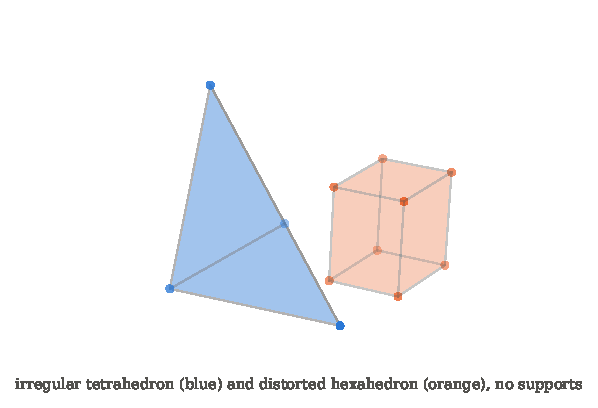
\includegraphics[width=0.4\textwidth]{fig_v_setup_v0.pdf}
\caption[V0d/V0e: boundary-value problem]{Boundary-value problem of V0d/V0e: one irregular tetrahedron and one distorted hexahedron, unconstrained.}
\label{fig:vsetup0}
\end{figure}

\trun \code{python -m tests.verify\_fe\_basics --ckpt checkpoints\slash{}phase1\_validated.pt --rve-ckpt <frozen.pt>}
\texpect Six zero eigenvalues, no negative ones, and a null space that contains
the six rigid-body vectors.
\tobtain See \cref{tab:v0d} and \cref{fig:v0spec}. The analytical law and the RVE pICNN pass in all
four element configurations: the rigid-body residual $\|\bm K\bm R\|$ is at
round-off, and the null space spans the rigid modes to $\le2\times10^{-9}$. The
legacy Phase~1 network, however, shows only \emph{three} zero eigenvalues and
\emph{three negative} ones. A rigid rotation of the unloaded body lowers its
energy. Evaluating the network directly confirms the cause predicted in
\cref{ch:theory}: for a rotation by $\theta$,
$\widehat\Psi(\Rten)=p_I\,(2-2\cos\theta)$ with $p_I=-0.2746$, to all printed
digits. This is the non-objective affine reference correction. It was removed
from Phase~5 onwards, which is why the production model passes. Tests V4--V6
could not detect the defect, because their Dirichlet boundaries suppress rigid
rotations. The Phase~1 gate verified the \emph{bridge}; it did not verify the
Phase~1 network as a frame-indifferent material.
\tinfer The assembly path produces the correct null space for the analytical law and for the production surrogate, so rigid motions cost no energy. The legacy Phase~1 network violates frame indifference and is therefore not a valid production model; this defect is invisible to tests with Dirichlet boundaries and is why the production energy is normalized objectively.

\begin{table}[H]
\centering\small
\caption[V0d/V0e: spectrum of the unconstrained element stiffness]{V0d/V0e: spectrum of the unconstrained element stiffness at $\F=\Iten$
(\code{assemble\_system}). $q$: NGSolve integration-rule order.}
\label{tab:v0d}
\begin{tabular}{@{}llrlrrrr@{}}
\toprule
Element & Order & $q$ & Material & DOFs & \#zero & \#neg. & $\|\bm K\bm R\|/(\|\bm K\|\|\bm R\|)$\\
\midrule
tet & 1 & 2 & neo-Hookean & 12 & 6 & 0 & $6.1\times10^{-17}$\\
tet & 1 & 2 & RVE pICNN & 12 & 6 & 0 & $5.7\times10^{-17}$\\
tet & 1 & 2 & Phase 1 pICNN (legacy) & 12 & \textbf{3} & \textbf{3} & $3.9\times10^{-3}$\\
tet & 2 & 4 & neo-Hookean / RVE pICNN & 30 & 6 & 0 & $\le1.2\times10^{-16}$\\
hex & 1 & 2 & neo-Hookean / RVE pICNN & 24 & 6 & 0 & $\le1.0\times10^{-16}$\\
hex & 2 & 4 & neo-Hookean / RVE pICNN & 81 & 6 & 0 & $\le2.5\times10^{-16}$\\
hex & 1 & 0 & neo-Hookean (one point) & 24 & \textbf{18} & 0 & $5.8\times10^{-17}$\\
\bottomrule
\end{tabular}
\end{table}

\begin{figure}[H]
\centering
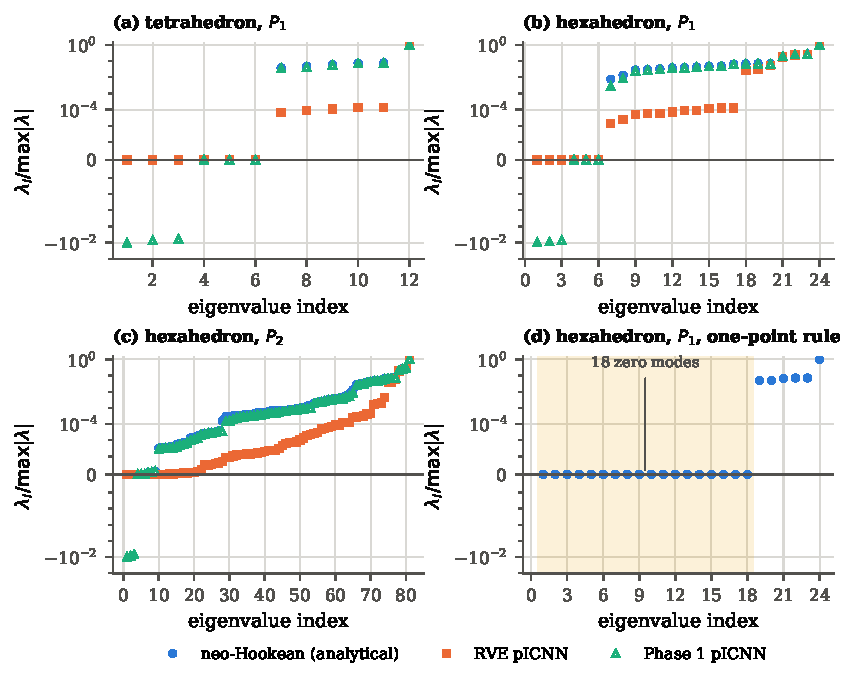
\includegraphics[width=\textwidth]{fig_v0_spectra.pdf}
\caption[V0d/V0e: sorted eigenvalues of the unconstrained element stiffness]{V0d/V0e: sorted eigenvalues of the unconstrained element stiffness at
$\F=\Iten$, normalized by the largest magnitude (symmetric-log axis). (a)--(c) Full
integration: six zero eigenvalues for the analytical law and the RVE pICNN; the
legacy Phase~1 network has three zero and three negative eigenvalues. The RVE
pICNN spectrum is shifted down because its largest eigenvalues are of order
$\kappa=10^4$. (d) One-point rule: 18 zero eigenvalues (6 rigid, 12 hourglass).}
\label{fig:v0spec}
\end{figure}

\testcase{V0e}{Under-integration and hourglass modes}
\taim Show that the test detects spurious zero-energy modes.
\tsetup The trilinear hexahedron of V0d with a one-point rule.
\texpect $6+12=18$ zero eigenvalues: 12 hourglass modes~\cite{Zienkiewicz2013}.
\tobtain 18 zero eigenvalues (\cref{fig:v0spec}d). Pass. With the full rule, V0d gives 6.
\tinfer The zero-mode test is sensitive enough to detect spurious modes: it finds exactly the twelve hourglass modes expected for one-point integration and none with the full rule used in production.

% ======================================================================
\section{Phase 1: PyTorch--NGSolve bridge}

Training labels come from \cref{eq:nh}. The tests add one layer of complexity at
a time. V1 checks the API: shapes $(4)$, $(4,3,3)$ and $(4,3,3,3,3)$, float64,
finite values, and agreement of the feature-level and material-level interfaces;
it passes. V2 checks the reference state: $|\widehat\Psi(\Iten)|=0$ and
$\max|P_{ij}(\Iten)|=0$, against a tolerance of $2.2\times10^{-15}$, while the raw
network has $|P_{\mathrm{raw}}(\Iten)|=1$; it passes.

\testcase{V2b}{Reproduction of the analytical response}
\taim Check that the trained Phase~1 network reproduces the neo-Hookean energy,
stress and tangent before it enters an FE solve.
\tsetup 256 admissible deformation gradients (seed 2026,
$|F_{ij}-\delta_{ij}|\le0.2$). Relative $L_2$ tolerances: 10\,\% (energy),
10\,\% (stress), 25\,\% (tangent).
\trun \code{python -m tests.verify\_neohooke\_response --ckpt checkpoints\slash{}phase1\_validated.pt}
\tobtain $5.367\,\%$, $3.274\,\%$ and $3.865\,\%$ (parity plots in \cref{fig:v2b}). Pass.
\tinfer The Phase~1 network reproduces the target law to a few percent, but not to the accuracy of the later checks; its remaining error (shear modulus $0.883$) must be kept in mind when V4--V8 are read as tests of the bridge, not of the material.

\begin{figure}[H]
\centering
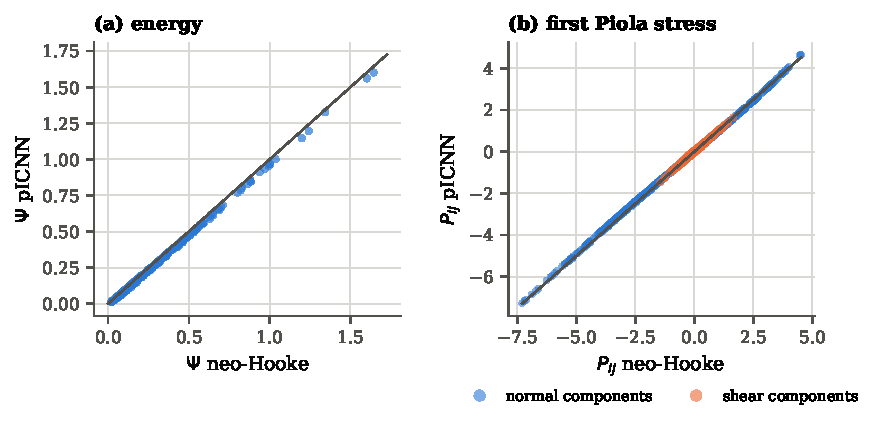
\includegraphics[width=0.9\textwidth]{fig_v2b.pdf}
\caption[V2b: Phase~1 network versus the neo-Hookean law]{V2b: Phase~1 network versus the analytical neo-Hookean law on 256 validation states. (a) Energy. (b) All components of the first Piola stress. Line: identity.}
\label{fig:v2b}
\end{figure}


\testcase{V3}{Automatic-differentiation tangent}
\taim Verify $\Aten=\partial\Pstress/\partial\F$ from AD against central
differences of $\Pstress$.
\tsetup Four seeded deformation gradients; $\epsilon=10^{-2},\dots,10^{-8}$.
Finite differences serve only as the check.
\trun \code{python -m tests.verify\_tangent}
\texpect A V-shaped error curve: truncation error $\propto\epsilon^2$ for large
$\epsilon$, round-off error $\propto\varepsilon_\mathrm{mach}/\epsilon$ for small
$\epsilon$; minimum below $10^{-6}$.
\tobtain \Cref{fig:v3}. The errors are $1.5\times10^{-5}$, $1.5\times10^{-9}$,
$2.3\times10^{-10}$ and $2.3\times10^{-8}$. The decrease by four decades per two
decades of $\epsilon$ confirms the $\epsilon^2$ truncation order. Pass.
\tinfer Automatic differentiation gives the exact tangent: the observed difference to central differences is entirely the truncation and round-off of the reference, with the expected $\epsilon^2$ slope. The finite-difference tangent of the original proposal could never match this accuracy.

\begin{figure}[H]
\centering
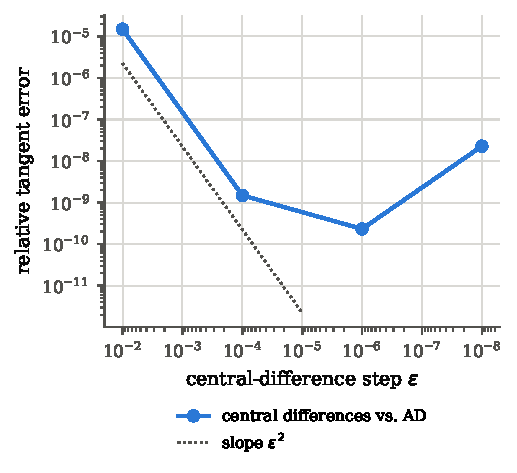
\includegraphics[width=0.5\textwidth]{fig_v3.pdf}
\caption[V3: central-difference error of the AD tangent]{V3: central-difference error of the AD tangent. It first decreases as $\epsilon^2$ (dotted guide) and then increases through round-off.}
\label{fig:v3}
\end{figure}


\testcase{V4}{Newton convergence of the nonlinear FE solve}
\taim Verify that the quadrature-point transfer and the consistent tangent
yield quadratic Newton convergence.
\tsetup Unit cube, $h=0.4$, $P_1$; $u_x=0.1x$ prescribed on $x=0$ and $x=1$;
trained Phase~1 network; tolerance $\|\bm R_\mathrm{free}\|<10^{-8}$.
\trun \code{python -m tests.verify\_element --ckpt checkpoints\slash{}phase1\_validated.pt}
\texpect $\|\bm R_{k+1}\|/\|\bm R_k\|^2$ bounded and the empirical order
\[q_k=\frac{\ln(r_{k+1}/r_k)}{\ln(r_k/r_{k-1})}\;\to\;2,\qquad r_k=\|\bm R_k\|.\]
\tobtain \Cref{tab:newton} and \cref{fig:v4}. Four iterations; the ratio stays
below 1 and $q$ rises to $1.90$. Quadratic convergence. Pass.
\tinfer The assembly, the quadrature-point transfer and the AD tangent are mutually consistent, because the Newton method converges with order close to two. A wrong tangent would reduce it to linear convergence.

\begin{figure}[H]
\centering
\begin{subfigure}[b]{0.42\textwidth}\centering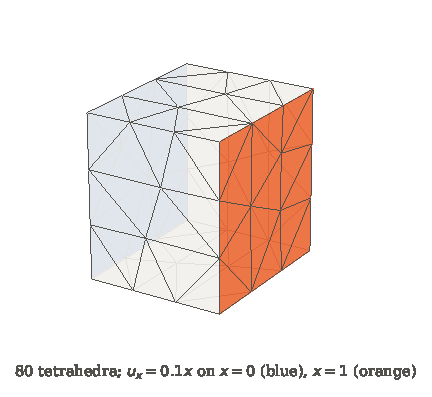
\includegraphics[width=\textwidth]{fig_v_setup_v4.pdf}\end{subfigure}\hfill
\begin{subfigure}[b]{0.55\textwidth}\centering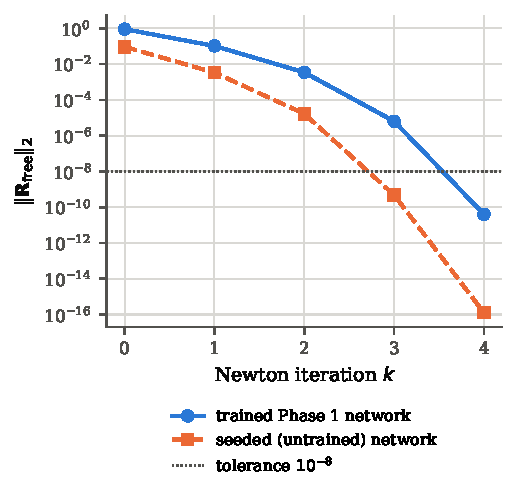
\includegraphics[width=\textwidth]{fig_v4.pdf}\end{subfigure}
\caption[V4: boundary-value problem and Newton residuals]{V4. (a) Boundary-value problem: unit cube, 80 tetrahedra, $u_x=0.1x$ on $x=0$ (blue, hidden) and $x=1$ (orange), lateral faces free. (b) Newton residuals of the trained and of an untrained (seeded) network.}
\label{fig:v4}
\end{figure}

\begin{table}[H]
\centering\small
\caption{V4: Newton residuals (tolerance $10^{-8}$).}
\label{tab:newton}
\begin{tabular}{@{}rccc@{}}
\toprule
$k$ & $\|\bm R_\mathrm{free}\|_2$ & $\|\bm R_{k+1}\|/\|\bm R_k\|^2$ & $q_k$\\
\midrule
0 & $9.058\times10^{-1}$ & 0.127 & --\\
1 & $1.043\times10^{-1}$ & 0.318 & 1.58\\
2 & $3.463\times10^{-3}$ & 0.535 & 1.85\\
3 & $6.412\times10^{-6}$ & 0.978 & 1.90\\
4 & $4.023\times10^{-11}$ & -- & --\\
\bottomrule
\end{tabular}
\end{table}

\testcase{V5}{Affine patch test}
\taim Verify that a homogeneous deformation is reproduced exactly on an
unstructured multi-element mesh through the full material path.
\tsetup Unit cube with 206 irregular tetrahedra (2884 material points). All boundary
nodes follow $\bm F_\mathrm{target}=\begin{bmatrix}1.08&0.05&0\\0&0.97&0.03\\0&0&1.02\end{bmatrix}$;
the interior nodes are free.
\begin{figure}[H]
\centering
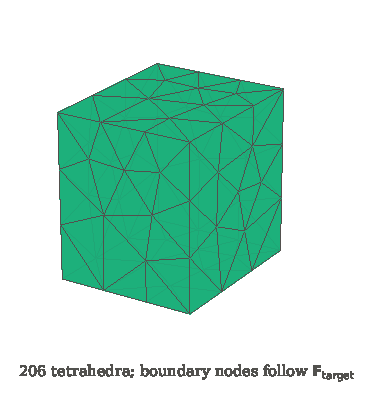
\includegraphics[width=0.33\textwidth]{fig_v_setup_v5.pdf}
\caption[V5: boundary-value problem]{Boundary-value problem of V5: unit cube with 206 tetrahedra; all boundary nodes follow $\bm F_\mathrm{target}$, interior nodes free.}
\label{fig:vsetup5}
\end{figure}

\trun \code{python -m tests.verify\_patch --ckpt checkpoints\slash{}phase1\_validated.pt}
\texpect Uniform $\F$ and $\Pstress$, and a vanishing free residual.
\tobtain $\max|\F-\bm F_\mathrm{target}|=4.4\times10^{-16}$, relative stress variation
$4.6\times10^{-15}$, $\|\bm R_\mathrm{free}\|=2.7\times10^{-16}$. Pass.
\tinfer The material path reproduces a homogeneous state exactly on an irregular mesh, so there is no spurious force from the transfer between the network and the finite-element space.

\testcase{V6}{Matched analytical and neural FE solutions}
\taim Compare complete nonlinear FE solutions obtained with the neural and the
analytical material.
\tsetup V4 geometry, $10\,\%$ stretch, lateral faces free; tolerance 15\,\% on
displacement, $\F$ and reaction vector.
\begin{figure}[H]
\centering
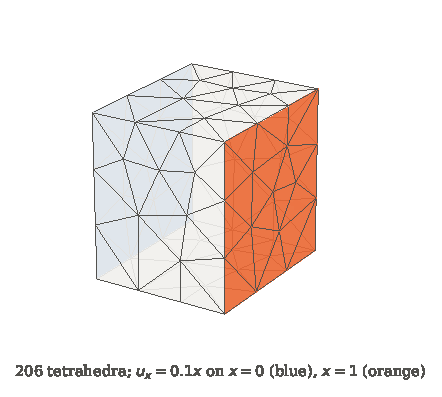
\includegraphics[width=0.33\textwidth]{fig_v_setup_v6.pdf}
\caption[V6: boundary-value problem]{Boundary-value problem of V6: unit cube with 206 tetrahedra, $u_x=0.1x$ on $x=0$ (blue, hidden) and $x=1$ (orange), lateral faces free.}
\label{fig:vsetup6}
\end{figure}

\trun \code{python -m tests.verify\_fe\_comparison --ckpt checkpoints\slash{}phase1\_validated.pt}
\tobtain Both solves converge in five iterations. The relative errors are
$2.00\,\%$ (displacement), $0.35\,\%$ ($\F$) and $13.4\,\%$ (reaction). Pass. The reaction error is close to its limit. Its origin is identified
by V8: the Phase~1 network has a small-strain shear modulus of $0.883$ instead of
$1$ ($-11.7\,\%$), although its relative stress error in V2b is only $3.3\,\%$.
\tinfer Network and analytical law give the same deformation field (displacement and $\F$ within $2\,\%$ and $0.4\,\%$); the larger reaction error is caused by the Phase~1 network's shear modulus and not by the bridge.

\testcase{V7}{Single element under full deformation control}
\taim Verify the constitutive response and the consistent tangent of one
element when every nodal degree of freedom is prescribed. Following the
guideline, the physically linear but geometrically nonlinear St.\ Venant--Kirchhoff
law, $\Psi=\tfrac{\lambda}{2}(\operatorname{tr}\bm E)^2+\mu\operatorname{tr}\bm E^2$, is
tested before the neo-Hookean law ($\mu=1$, $\lambda=10$).
\tsetup One trilinear hexahedron (unit cube, $2\times2\times2$ Gauss rule). All nodes
follow the affine map of the non-symmetric
$\Fbar=\begin{bmatrix}1.10&0.06&-0.02\\0.03&0.92&0.05\\-0.04&0.02&1.05\end{bmatrix}$.
The assembled stiffness $\bm K$ (production \code{assemble\_system}) is compared with
central differences of the assembled residual along a random direction.
\trun \code{python -m tests.verify\_stress\_control}
\texpect $\F=\Fbar$ and $\Pstress=\Pstress^{\mathrm{analytic}}(\Fbar)$ at every Gauss point to
round-off; tangent error $\propto\epsilon^2$ until round-off.
\tobtain $\max|\F-\Fbar|=2.4\times10^{-16}$; relative stress error $5.5\times10^{-15}$
(SVK) and $3.4\times10^{-15}$ (neo-Hooke). Tangent errors fall from $8.5\times10^{-6}$
($\epsilon=10^{-3}$) to $1.7\times10^{-11}$ ($\epsilon=10^{-6}$) for SVK, and from
$3.5\times10^{-6}$ to $1.8\times10^{-11}$ for neo-Hooke, decreasing by two decades per decade of $\epsilon$
(\cref{fig:v7}). Pass.
\tinfer The constitutive response and the assembled tangent are correct for a general, non-symmetric $\Fbar$ including the geometric nonlinearity; the tangent error is limited only by the difference step.

\begin{figure}[H]
\centering
\begin{subfigure}[b]{0.42\textwidth}\centering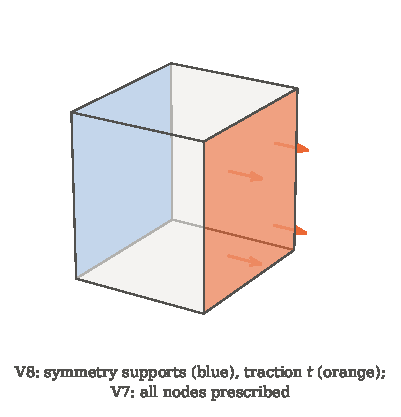
\includegraphics[width=\textwidth]{fig_v_setup_v78.pdf}\end{subfigure}\hfill
\begin{subfigure}[b]{0.55\textwidth}\centering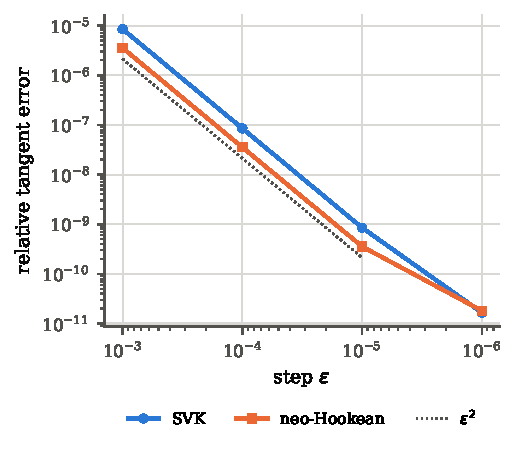
\includegraphics[width=\textwidth]{fig_v7.pdf}\end{subfigure}
\caption[V7/V8: boundary-value problems and V7 tangent error]{V7 and V8. (a) Boundary-value problems of the single trilinear hexahedron. V7: all nodes prescribed by the affine map. V8: symmetry supports on $x=0$, $y=0$, $z=0$ (blue) and nominal traction $t$ on $x=1$ (orange). (b) V7: error of the assembled tangent against central differences of the residual (SVK and neo-Hooke); dotted: slope $\epsilon^2$.}
\label{fig:v7}
\end{figure}


\testcase{V8}{Single element under stress control}
\taim Verify the solver under prescribed tractions (Neumann boundary
conditions) with only the minimal supports, including quadratic Newton
convergence in every load step.
\tsetup The same hexahedron with symmetry supports $u_x=0$ on $x=0$, $u_y=0$ on $y=0$
and $u_z=0$ on $z=0$; dead-load nominal traction $(t,0,0)$ on $x=1$, increased to
$t=0.6$ in three steps; all other faces free. The reference solution
$\F=\operatorname{diag}(a,b,b)$ is computed independently from $P_{11}=t$,
$P_{22}=P_{33}=0$. Tractions and component-wise supports are options of the production solver \code{solve}.
\trun \code{python -m tests.verify\_stress\_control --ckpt checkpoints/phase1\_validated.pt}
\texpect Homogeneous FE solution with $F_{11}=a$, $F_{22}=F_{33}=b$ and
$\Pstress=\operatorname{diag}(t,0,0)$ to round-off; quadratic Newton convergence.
\tobtain \Cref{tab:v8} and \cref{fig:v8}. For both analytical laws the stretches agree with the
reference to $\le2.4\times10^{-15}$ and $|\Pstress-\operatorname{diag}(t,0,0)|/t\le1.4\times10^{-14}$;
each load step converges in four Newton iterations with an empirical order of about
2 (for example $10^{-1}\to3.7\times10^{-2}\to1.4\times10^{-4}\to2.6\times10^{-8}\to7.8\times10^{-16}$
for neo-Hooke at $t=0.6$). Pass. The trained Phase~1 network, run through the same
test for comparison, satisfies equilibrium ($|\Pstress-\operatorname{diag}(t,0,0)|/t=10^{-12}$),
but its stretches deviate from neo-Hooke by $+17.8\,\%$ of the axial stretch increment at
$t=0.2$ and by $+31\,\%$ at $t=0.6$, where $a=1.25$ also exceeds the Phase~1 training
range. The cause is its shear modulus of $0.883$, a constitutive (not a solver) error.
\tinfer The solver handles prescribed tractions with minimal supports and converges quadratically in every step. The deviation of the Phase~1 network from the neo-Hookean law is a property of the network, which confirms the shear-modulus defect found in V6.

\begin{figure}[H]
\centering
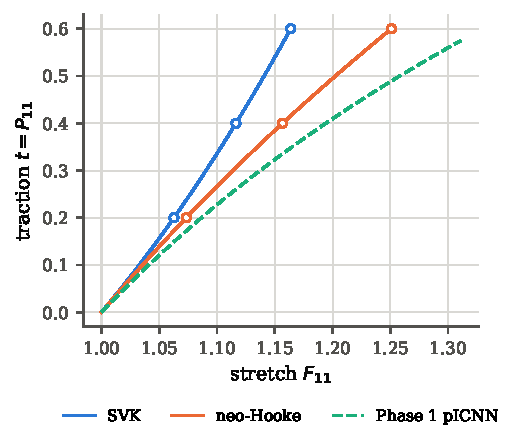
\includegraphics[width=0.5\textwidth]{fig_v8.pdf}
\caption[V8: uniaxial nominal traction versus axial stretch]{V8: uniaxial nominal traction versus axial stretch. Lines: independent reference solution of $P_{11}=t$, $P_{22}=P_{33}=0$; circles: FE solution after each load step (agreement to $\le2.4\times10^{-15}$). The Phase~1 network is softer than the neo-Hookean law it was trained on.}
\label{fig:v8}
\end{figure}

\begin{table}[H]
\centering\small
\caption{V8: uniaxial stress control of one hexahedron at $t=0.6$.}
\label{tab:v8}
\setlength{\tabcolsep}{4pt}
\begin{tabular}{@{}lcccc@{}}
\toprule
Material & reference $a$ / $b$ & $\max|F_{11}-a|$ & $\max|F_{22,33}-b|$ & it./step\\
\midrule
St.\ Venant--Kirchhoff & 1.1638045 / 0.9159096 & $1.3\times10^{-15}$ & $1.6\times10^{-15}$ & 4\\
neo-Hooke & 1.2509757 / 0.9024160 & $2.4\times10^{-15}$ & $1.9\times10^{-15}$ & 4\\
Phase~1 pICNN & as neo-Hooke & $7.9\times10^{-2}$ & $5.3\times10^{-2}$ & 4\\
\bottomrule
\end{tabular}
\end{table}

% ======================================================================
\section{Phase 2: periodic RVE and homogenization}

The tests run on reduced meshes ($h=0.22$--$0.35$). Each prints its metrics and a
PASS line.

\testcase{P2-V1}{Periodic space}
\taim Opposite faces must carry identical fluctuation values.
\tsetup Periodic $P_2$ space on the cell with cavity (371 elements).
\trun \code{python -m tests.verify\_periodic\_rve}
\tobtain 2208 unconstrained active DOFs are reduced to 1485 (723 eliminated). The
maximum opposite-face jump is $2.2\times10^{-16}$. Pass.
\tinfer The periodic space is exactly triply periodic, so no spurious boundary stress enters the RVE solution.

\testcase{P2-V2}{Rigid kinematics}
\taim The prescribed cavity trace must be an exact rigid motion: six independent
modes, and proper rotations at finite angles.
\trun \code{python -m tests.verify\_rigid\_particle}
\tobtain Distance error $1.1\times10^{-16}$; rigid-map rank 6; constraint residual
$7.2\times10^{-18}$; linearization error of the rotation increment
$7.7\times10^{-10}$. Pass.
\tinfer The rigid particle is exactly rigid and its rotation is a proper rotation, so the penalty parameter of the proposal is no longer needed.

\testcase{P2-V3}{Mixed patch at $\kappa/\mu=10^4$}
\taim The Taylor--Hood formulation must reproduce a homogeneous finite deformation
exactly, without volumetric locking.
\trun \code{python -m tests.verify\_mixed\_matrix}
\tobtain Errors in $\F$, $J$ and $p$ of $2.3\times10^{-15}$, $2.2\times10^{-15}$ and
$2.9\times10^{-13}$; pressure variation $3.6\times10^{-15}$; final residual
$6.3\times10^{-16}$. Pass.
\tinfer The Taylor--Hood pair is free of volumetric locking at $\kappa/\mu=10^4$, which is what allows the RVE to represent the near-incompressible matrix.

\testcase{P2-V4}{Coupled periodic RVE}
\taim The periodic matrix and the rigid particle must be in equilibrium together.
\trun \code{python -m tests.verify\_coupled\_rve}
\tobtain Rigid-trace error $8.0\times10^{-19}$; relative particle force and moment
$2.1\times10^{-7}$ and $7.4\times10^{-9}$ (prescribed rotation); final residual
$1.9\times10^{-14}$. Pass.
\tinfer Matrix and particle are in equilibrium, and the periodic jump and the rigid trace are exact to round-off; the particle force and moment are small but not machine zero because the rotation is prescribed in this test.

\testcase{P2-V5}{Hill--Mandel macro-homogeneity}
\taim The homogenized stress \cref{eq:hm} must be work-conjugate to $\Fbar$.
\tsetup Finite hydrostatic loading of the cell; mixed $P_2/P_1$, $\kappa/\mu=10^4$.
Macroscopic and microscopic virtual powers are compared for independent virtual
rates. A constant-stress recovery checks sign, index order and volume
normalization.
\trun \code{python -m tests.verify\_hill\_mandel}
\texpect Equal powers to round-off.
\tobtain Microscopic and macroscopic power are both $470.9456611477$; relative error
$1.2\times10^{-15}$; alternative virtual field $1.4\times10^{-15}$; constant-stress
recovery $4.0\times10^{-14}$. The raw boundary-traction estimate, kept as a
diagnostic, is off by $3.9\times10^{-6}$. This confirms that the reaction term in
\cref{eq:hm} is necessary. Pass.
\tinfer The reaction-based homogenized stress satisfies the Hill--Mandel condition, whereas the naive boundary-traction estimate is wrong at the $10^{-6}$ level; the reaction term is therefore required.

\testcase{P2-V6}{Condensed homogenized tangent}
\taim Verify \cref{eq:schur}: major symmetry, consistency with the stress, and
second-order Taylor remainder.
\tsetup Cell with prescribed particle rotation (1472 elements), loaded off the
identity. Remainder $r(t)=\|\Pbar(\Fbar+t\bm D)-\Pbar(\Fbar)-t\Abar:\bm D\|$ for
$t=10^{-3},5\times10^{-4},2.5\times10^{-4}$, re-solving the RVE at each step.
\trun \code{python -m tests.verify\_homogenized\_tangent}
\texpect $r\propto t^2$, that is, observed order 2.
\tobtain (\cref{fig:vp2v6}) $r=6.760\times10^{-3}$, $1.690\times10^{-3}$, $4.225\times10^{-4}$, giving
orders $2.000$ and $2.000$. Symmetry error $3.0\times10^{-16}$; energy-gradient
stress error $6.7\times10^{-16}$; independent sensitivity error
$1.7\times10^{-15}$. Pass.
\tinfer The condensed tangent is exact: it is the derivative of the stress, it is symmetric, and the second-order Taylor remainder shows that no first-order error is present.

\begin{figure}[H]
\centering
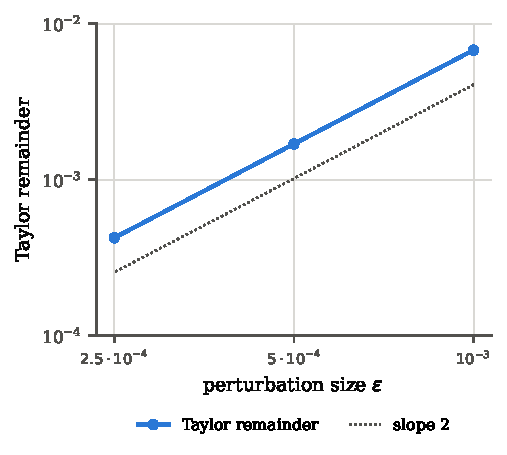
\includegraphics[width=0.5\textwidth]{fig_v_p2v6.pdf}
\caption[P2-V6: Taylor remainder of the condensed RVE tangent]{P2-V6: Taylor remainder of the condensed RVE tangent versus perturbation size; dotted: slope 2.}
\label{fig:vp2v6}
\end{figure}


\testcase{P2-V7}{Free finite particle rotation}
\taim Under simple shear ($\gamma=0.05$) the free particle must rotate until its
resultant moment vanishes, while $\Rten$ stays a proper rotation.
\trun \code{python -m tests.verify\_free\_rotation}
\tobtain Three outer Newton iterations reduce the moment residual from
$4.75\times10^{-3}$ to $8.0\times10^{-16}$. The particle rotates by
$-0.0249\,$rad about $z$. Orthogonality error $2.5\times10^{-16}$; determinant error
$4.4\times10^{-16}$; rotational-Hessian symmetry $1.3\times10^{-17}$. Pass.
\tinfer The free rotation is determined by moment equilibrium within three outer iterations, with proper orthogonality, so the particle can be treated as freely rotating at no extra modelling error.

\testcase{P2-V8}{Translation gauge}
\taim A common translation of the fluctuation and the particle must leave all
physical fields unchanged.
\trun \code{python -m tests.verify\_translation\_gauge}
\tobtain For a shift of $2.7\times10^{-3}$, the changes in $\F$, $p$, pointwise stress and
homogenized stress are $1.1\times10^{-15}$, $4.0\times10^{-15}$, $8.9\times10^{-15}$ and
$1.2\times10^{-15}$. Pass.
\tinfer The translation of the particle is a pure gauge, which justifies fixing it without changing any physical result.

\testcase{P2-V9}{Free-rotation homogenized tangent against re-solved central differences}\label{sec:p2v9}
\taim Verify the complete production tangent of the freely rotating particle,
including rotational condensation, against the strongest possible reference:
central differences in which the full nonlinear RVE, including the rotation
equilibrium, is \emph{re-solved} at every perturbed macroscopic state.
\tsetup Pilot record \code{v001\_f000047} ($\vfrac=0.05$, $J_{\min}=0.65$ and
$J_{\max}=1.59$ inside the cell), production settings ($h=0.22$, $P_2/P_1$,
integration order 10). Step $10^{-4}$ in all nine row-major directions of $\Fbar$, that
is $1+18$ full RVE solves, plus objectivity re-solves under rotated $\Fbar$.
\trun \code{python -m benchmarks.rve\_constitutive\_checks --dataset <pilot.npz> --output p2v9.json --sample-ids v001\_f000047}
\texpect Agreement within the stored tolerances: tangent $5\times10^{-3}$, energy gradient
$5\times10^{-4}$, stress $5\times10^{-5}$, objectivity $10^{-6}$ (energy).
\tobtain Status \emph{pass}, after $59.6\,$min on one core. The maximum
directional tangent error is $5.2\times10^{-12}$ and the maximum energy-gradient
error $1.8\times10^{-11}$. Base-stress work versus condensed stress agrees to
$7.6\times10^{-16}$; objectivity errors are $1.3\times10^{-15}$ (energy) and
$1.2\times10^{-15}$ (stress). The equilibrium residuals are $1.3\times10^{-13}$
(mixed), $6.5\times10^{-15}$ (rotation) and $6.2\times10^{-13}$ (condensed). The free-rotation tangent is
therefore exact to the accuracy of the re-solved differences.
\tinfer The full free-rotation tangent, including the condensation of the rotation, agrees with finite differences of re-solved RVEs to the accuracy of the differences; it is therefore exact and can be used by a Newton solver.


\testcase{P2-V10}{Dataset contract}
\taim Generation must be deterministic and splits must be leak-free.
\trun \code{python -m tests.verify\_rve\_dataset}
\tobtain 12 states at two volume fractions; regeneration error $0$; zero cross-split
leaks; a different seed changes the states (by $0.28$); serialization error $0$;
tangent shape $(9,9)$. Pass.
\tinfer Datasets are reproducible and the splits do not leak, so the test statistics of \cref{ch:assessment} are not contaminated by overlapping states.

% ======================================================================
\paragraph{Newton convergence across all solvers.} \Cref{fig:vnewton} collects the
residual histories of every nonlinear solve in the test suite: the Phase~1 bridge
(V4, V6), the single hexahedron under stress control (V8), the mixed patch
(P2-V3), the coupled RVE (P2-V4), the outer rotation iteration (P2-V7) and the
first load increment of the macroscopic problem (M-V0). All show the
characteristic quadratic tail, with the number of correct digits roughly doubling
in each of the last iterations. Since each solver uses its own exact or AD
Jacobian, this is a joint check of all tangents in the code. \Cref{fig:vrvechecks}
summarizes the identities checked by the RVE tests.

\begin{figure}[H]
\centering
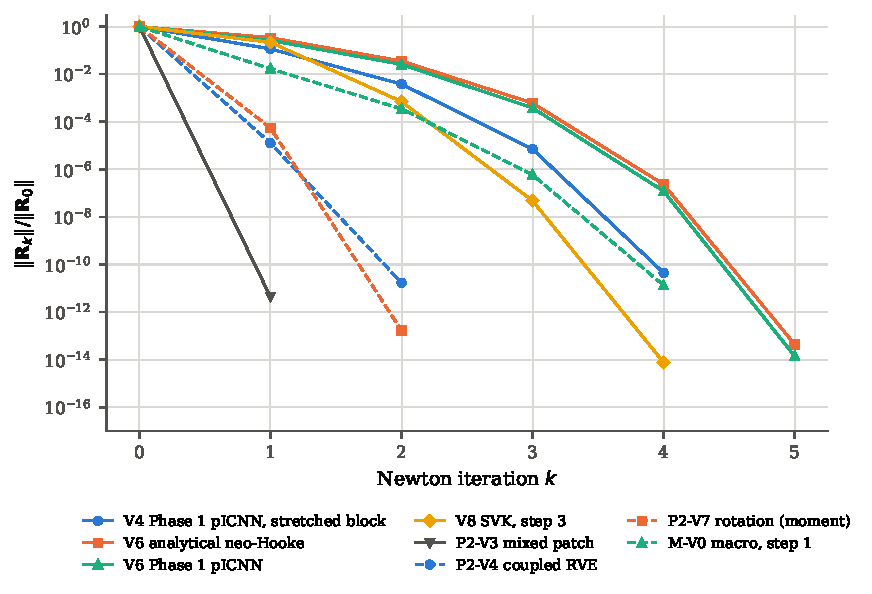
\includegraphics[width=0.95\textwidth]{fig_v_newton_all.pdf}
\caption[Normalized Newton residuals of all nonlinear solves]{Normalized Newton residuals of all nonlinear solves in the test suite. P2-V3 ($J=1.001$) converges in one step.}
\label{fig:vnewton}
\end{figure}

\begin{figure}[H]
\centering
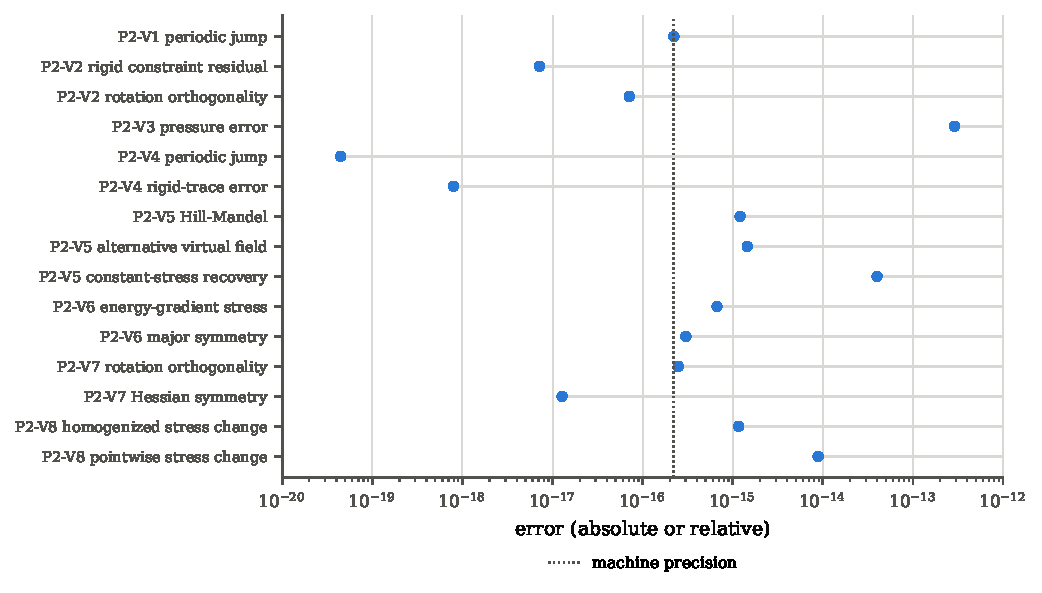
\includegraphics[width=0.95\textwidth]{fig_v_rve_checks.pdf}
\caption[Identities checked by the RVE tests P2-V1 to P2-V8]{Identities checked by the RVE tests P2-V1 to P2-V8 (absolute or relative errors as printed by the tests); dotted: machine precision.}
\label{fig:vrvechecks}
\end{figure}

\section{Surrogate and macroscopic tangent checks}

\testcase{S-V1}{Constitutive consistency of the trained surrogate}
\taim For an RVE-trained checkpoint, check on held-out states that
$\partial\widehat\Psi/\partial\F$ equals the returned stress and that the
tangent equals directional differences of the stress, and check objectivity
($\widehat\Psi(\bm Q\F)=\widehat\Psi(\F)$) and major symmetry.
\tsetup 36 records (12 states, three volume fractions), central differences with
step $10^{-5}$, thresholds $10^{-6}$ (gradient), $10^{-5}$ (tangent), $10^{-10}$
(objectivity).
\trun \code{python -m benchmarks.rve\_surrogate\_constitutive\_checks --dataset <phase7.npz> ...} (\cref{ch:manual})
\tobtain Frozen checkpoint: status \emph{pass} for 36 records (\cref{fig:vs1});
energy gradient $4.9\times10^{-8}$, tangent $1.0\times10^{-9}$, objectivity
$4.8\times10^{-13}$ (energy) and $1.7\times10^{-12}$ (stress), symmetry $6.0\times10^{-16}$.
During development the same test \emph{failed} for the Phase~5
checkpoint (objectivity energy error $0.91$), which led to the objective correction
\cref{eq:norm}. The test thus detected a physical defect that an accuracy metric
could not reveal.
\tinfer Stress and tangent of the surrogate are exact derivatives of its energy, and the energy is objective and symmetric on held-out states. The surrogate is thus a valid hyperelastic law; its remaining deficit (\cref{ch:assessment}) is accuracy, not consistency.

\begin{figure}[H]
\centering
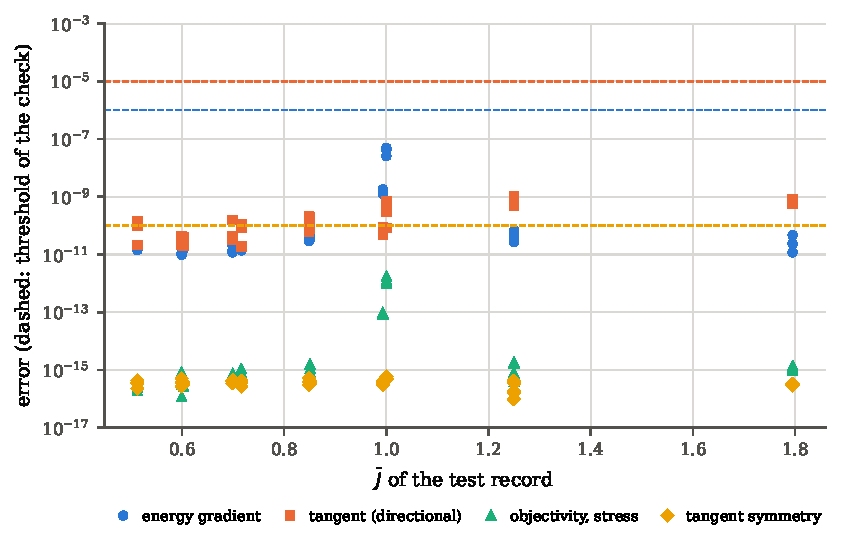
\includegraphics[width=0.95\textwidth]{fig_v_s1.pdf}
\caption[S-V1: errors of the frozen surrogate for the audited records]{S-V1: errors of the frozen surrogate for the 36 audited test records versus $\overline J$; dashed lines: thresholds of the corresponding checks (same colour).}
\label{fig:vs1}
\end{figure}


\testcase{M-V0}{Macroscopic tangent consistency}
\taim Verify the assembled global stiffness of the macro problem against
directional differences of the residual at a non-equilibrium iterate.
\trun \code{python -m benchmarks.phase6\_macro\_fe\_demo --tangent-check-only ...}; full command in \code{tests/README.md}
\tobtain Frozen checkpoint ($P_1$, $h=0.25$, predictor state of the
second increment at $1\,\%$ stretch): relative directional error $6.5\times10^{-10}$;
symmetry error $1.5\times10^{-16}$; Newton linear solve accurate to $5.1\times10^{-16}$.
The free stiffness has eigenvalues of magnitude $0.44$ to $1.46\times10^4$, a condition
estimate of $3.3\times10^4$, of the order of $\kappa/\mu=10^4$, and one negative eigenvalue at this
non-equilibrium predictor state. This is the conditioning that governs the
macroscopic solver behaviour discussed in \cref{sec:macro}.
\tinfer The assembled macroscopic tangent is consistent with the residual, so any slow macroscopic convergence stems from the conditioning and the nonlinear path, not from a faulty Jacobian.
